\documentclass[nobib]{tufte-handout}

\title{Privacy Tools for Data Sharing}
\author[Stephen Weis]{Stephen Weis}

\date{January 2020} % without \date command, current date is supplied

%\geometry{showframe} % display margins for debugging page layout

\usepackage{graphicx} % allow embedded images
  \setkeys{Gin}{width=\linewidth,totalheight=\textheight,keepaspectratio}
  \graphicspath{{graphics/}} % set of paths to search for images
\usepackage{amsmath}  % extended mathematics
\usepackage{booktabs} % book-quality tables
\usepackage{units}    % non-stacked fractions and better unit spacing
\usepackage{multicol} % multiple column layout facilities
\usepackage{lipsum}   % filler text
\usepackage{fancyvrb} % extended verbatim environments
  \fvset{fontsize=\normalsize} % default font size for fancy-verbatim environments

%\usepackage{draftwatermark}

% Standardize command font styles and environments
\newcommand{\doccmd}[1]{\texttt{\textbackslash#1}} % command name -- adds backslash automatically
\newcommand{\docopt}[1]{\ensuremath{\langle}\textrm{\textit{#1}}\ensuremath{\rangle}} % optional command argument
\newcommand{\docarg}[1]{\textrm{\textit{#1}}} % (required) command argument
\newcommand{\docenv}[1]{\textsf{#1}} % environment name
\newcommand{\docpkg}[1]{\texttt{#1}} % package name
\newcommand{\doccls}[1]{\texttt{#1}} % document class name
\newcommand{\docclsopt}[1]{\texttt{#1}} % document class option name
\newenvironment{docspec}{\begin{quote}\noindent}{\end{quote}} % command specification environment

\begin{document}

\maketitle % this prints the handout title, author, and date

\begin{abstract}

\noindent This is an overview about common tools and definitions
for anonymizing data or confidentially computing over private data.
It is roughly in order of practicality and maturity and is summarized in a
table at the end.
\end{abstract}

\section{Information Reduction Techniques}

\textbf{Minimization} refers to collecting the minimal data necessary for
a specific purpose. \textbf{Redaction} deletes or censors data which has
already been collected.

\textbf{Aggregation} reduces a set of individual values to a smaller set of
derived values, for example, summing or averaging a list of values into a single
number. Training machine learning models or projecting high-dimensional data to
lower dimensions are also forms of aggregation.

\begin{marginfigure} 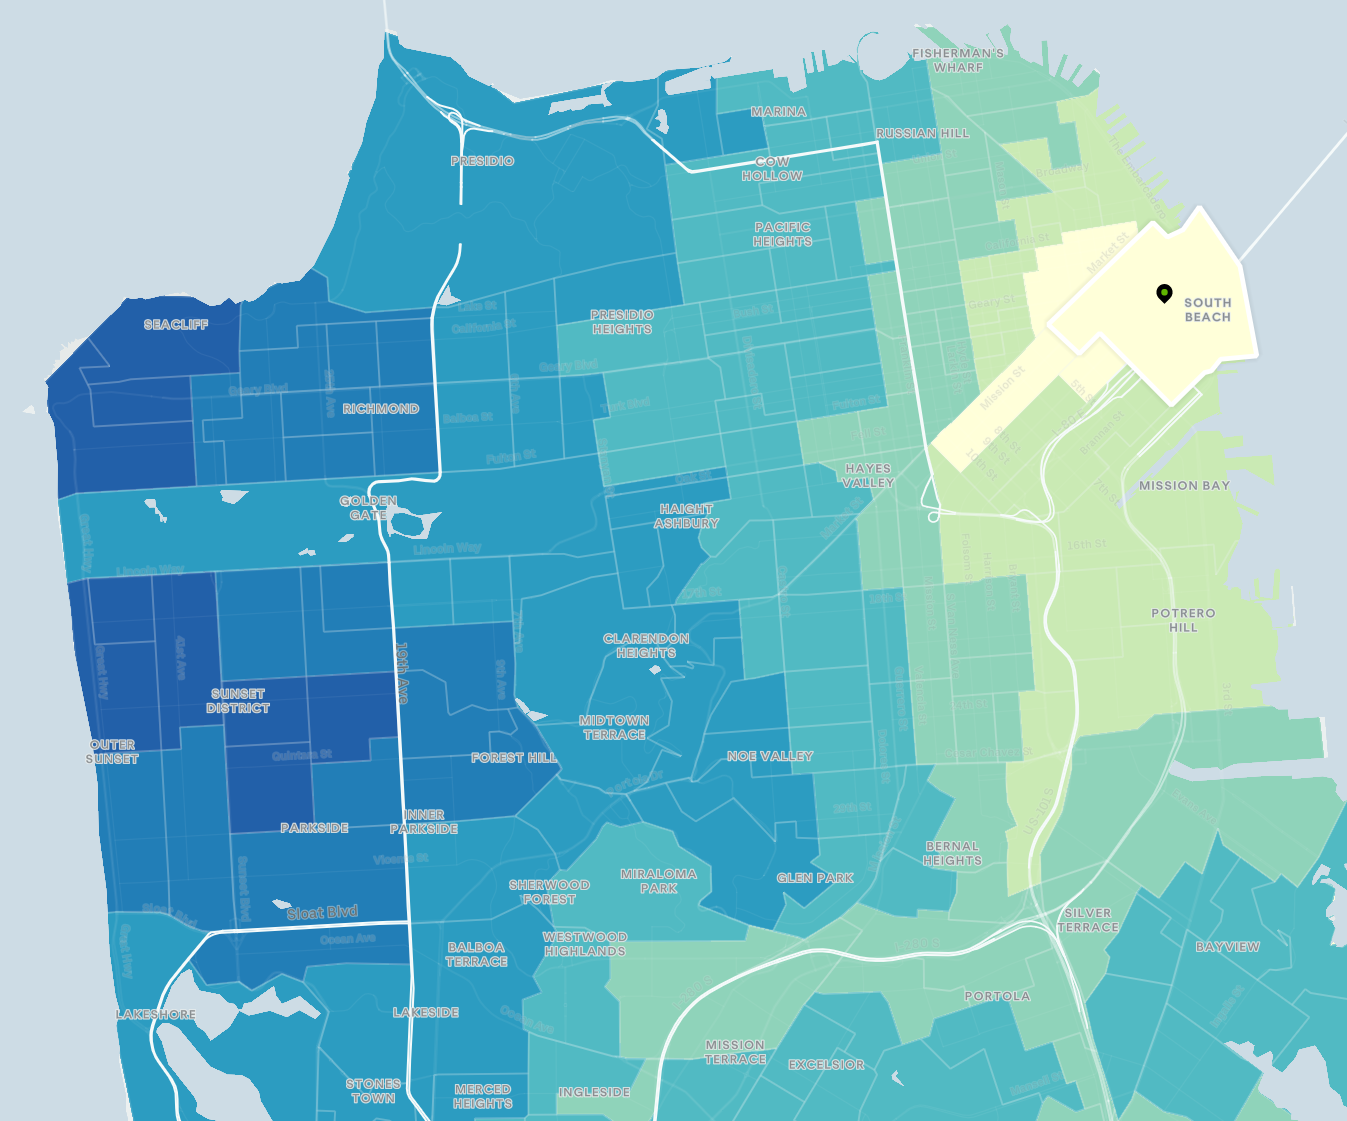
\includegraphics[width=\linewidth]{binned}
\caption{An example map of aggregated geolocation data, binned by neighborhood
and time.}
\label{fig:binned} \end{marginfigure}

\textbf{Binning} or \textbf{bucketing} is a common form of aggregation that
groups values into buckets or ranges through rounding, truncation, or some
other mapping. Examples might include truncating GPS coordinates to 3 decimal
places or rounding time values to the nearest 15 minute period.

\textbf{Top-coding} and \textbf{bottom-coding} are both types of binning which
group together the tail ends of distributions, where there may be few samples.
For instance, grouping ages of "Under 20", "20-45", "46-65", "Over 65" uses both
bottom- and top-coding for the respective youngest and oldest groups.

One concern with aggregation are \textbf{differencing attacks} which compare two
aggregated values for different sets and extract the different individual input
values. For example, given the average of Alice and Bob’s salary (e.g. \$50k)
and the average of Alice, Bob, and Carol’s salary (\$60k), you can learn
Carol’s salary (\$80k). Data sets which differ in individual values are
called \textbf{neighboring data}.

\section{k-Anonymity and Extensions}

Implicit in binning values for privacy is the notion of
\textit{safety in numbers} -- that grouping an individual with others will hide
that person's identity. The notion of \textbf{$k$-anonymity}
\cite{DBLP:journals/ijufks/Sweene02} is that at least $k$ people will be in any
given bin or group. Aggregated data, APIs, or visualization tools often have
\textbf{minimum thresholds} before returning data, so are $k$-anonymous in
practice. Google often uses $k$ values of 1000 in their advertising and
analytics products. Facebook has used $k$ values of 20 for advertising products.
Some government agencies use minimum thresholds of 3 before showing data.

The privacy provided by $k$-anonymity depends on the underlying data set. One
problem is \textbf{homogenous data}, where every member of a bin has a common
sensitive trait. In Figure \ref{fig:kanon}, we know all 30-40 year olds were
diagnosed with cancer.

A second problem is deanonymizing people by joining \textbf{background
knowledge} to a $k$-anonymous data set. For example, again in Figure
\ref{fig:kanon}, one may know the incidence rate of specific diseases across
different nationalities. That could be used to infer the nationality of a given
record, which had been redacted.

\begin{marginfigure} 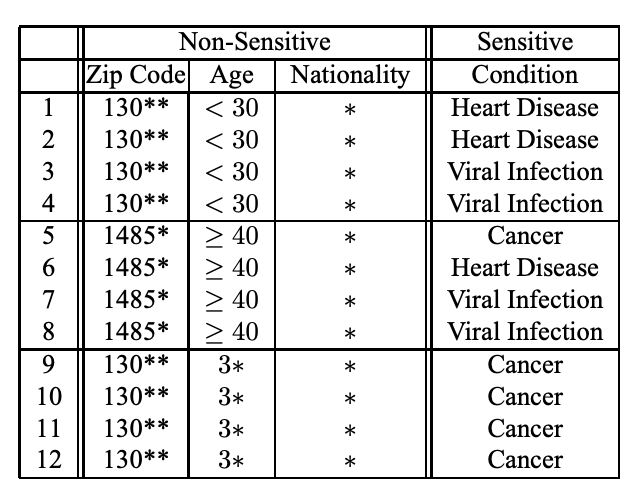
\includegraphics[width=\linewidth]{kanon}
\caption{A 4-anonymous table. Zip codes have been truncated, ages have been
top- and bottom-coded, and nationalities have been redacted so that each
(zip code, age range) has 4 records associated with it. Source:
\cite{DBLP:conf/icde/MachanavajjhalaGKV06}}
\label{fig:kanon} \end{marginfigure}

\textbf{$L$-diversity} \cite{DBLP:conf/icde/MachanavajjhalaGKV06} is an extension
of $k$-anonymity that addresses the homogeneity issue by ensuring that sensitive
traits among bins have at least $l$ distinct values. \textbf{$T$-closeness}
\cite{DBLP:conf/icde/LiLV07} is a further refinement that ensures that those
distinct values are distributed similarly to the population that data are drawn
from. Neither $l$-diversity nor $t$-closeness are widely used in practice,
though Google offers an $l$-diversity measurement in their data loss prevention
API \cite{google-risk-analysis}.

\section{Pseudonymization and Tokenization}

\textbf{Pseudonymization} or \textbf{tokenization} mean replacing sensitive
values like names, credit card numbers, or phone numbers with surrogate or token
values. These tokens retain their original relationship in the data set and are
often used as database lookup keys.

Tokenization often uses a \textbf{lookup table with random values} or
universally unique identifiers (UUIDs) mapping to original values. This has the
strongest security guarantee, but requires storing an entire mapping of the
original data to token values.

\textbf{Pseudorandom functions} (PRFs) are functions that take a secret key and
arbitrary data as input, and output fixed-length values indistinguishable from
randomness. Rather than storing an entire table of random tokens, one can use a
PRF to tokenize data with only a secret key. HMACs like HMAC-SHA256 are often
used as PRFs in practice.

\textbf{Format preserving encryption} \cite{DBLP:conf/sacrypt/BellareRRS09}
(FPE) entails encrypting sensitive fields such that the output ciphertext has
the same format as the input. For example, an format-preserving encrypted credit
card could have 16 decimal digits. FPE allows ciphertexts to be stored in
existing data fields, like database columns, which may not be easily changed.
FPE is also advantageous because, unlike PRFs, the original input data can be
decrypted with the secret key. AES FFX mode \cite{dworkin2016recommendation}
is one recent standard for FPE encryption.

%\begin{marginfigure}
%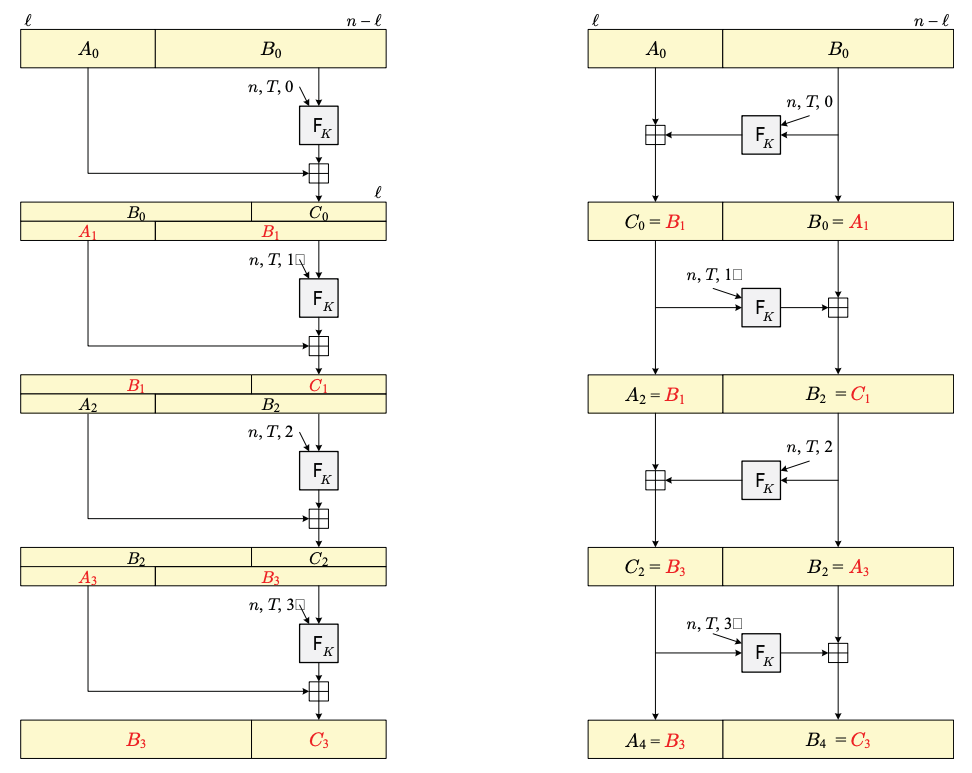
\includegraphics[width=\linewidth]{ffx}
%\caption{Illustration of the FFX format preserving encryption mode} \label{fig:ffx}
%\end{marginfigure}

Historically, \textbf{one-way functions} have often been misused for
pseudonymization. Many examples of re-identification have occurred when someone
naively used a hash function like MD5 or SHA-1 and stored the digests without
salting the input. Hash functions are not keyed like PRFs. Rather, anyone can
compute them.

The risk of unkeyed hash functions is if the input values have low entropy or
are from a known set. That allows someone to conduct a \textbf{dictionary
attack} where they simple try hashing many values or use precomputed known hash
values available online. Developers often try to avoid this by including an ad
hoc salt value. In general, simply hashing should be avoided unless the input is
known to be high-entropy.

\section{Differential Privacy}

\textbf{Differential privacy} defines the amount of information about an
individual which could be leaked from a dataset \cite{dwork2014algorithmic}.
Differential privacy is used by the US Census \cite{census-differential-privacy},
Apple \cite{apple-differential-privacy}, Google \cite{google-differential-privacy},
Facebook \cite{facebook-url-release}, and Uber \cite{uber-differential-privacy}
to protect research and user data.

Fundamentally, achieving differential privacy means adding some form of noise or
randomization while sacrificing accuracy. In its most basic form, differential
privacy specifies a numerical bound, $\epsilon$, on how much an
algorithm’s output can change between two neighboring datasets that only differ
in a single element. Part of the value of differential privacy is that
$\epsilon$-private systems can be composed with easily understood properties.
This lets one set a \textbf{privacy budget} and allow queries until that
budget is exhausted.

A \textbf{privacy mechanism} is an implementation that achieves a target
$\epsilon$-privacy. A simple mechanism is \textbf{randomized response}, which
was designed to allow people to answer surveys about sensitive topics. The idea
is that you flip a coin \textit{Heads} to either answer honestly 
(e.g. \textit{“Did you cheat on your taxes?”}) or \textit{Tails} to commit to
the answer with negative connotations (\textit{“Yes”}). This gives the survey
taker plausible deniability that they simply flipped a \textit{Tails}. It is
also easy to subtract the estimated noise and approximate the true answer rate.

Another privacy mechanism is the \textbf{Laplace Mechanism}, which adds randomly
sampled noise from the Laplace distribution, shown in Figure \ref{fig:laplace}.
This is a simple mechanism that is tunable to achieve any chosen level of
$\epsilon$-privacy and does not depend on the domain of the input data.

\begin{marginfigure} 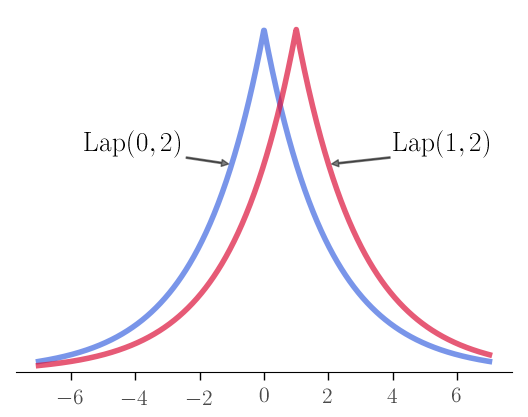
\includegraphics[width=\linewidth]{laplace}
\caption{Example of a Laplace distributions offering .5-differential privacy for
a function with sensitivity 1.} \label{fig:laplace} \end{marginfigure}

\textbf{Local differential privacy} refers to applying a privacy mechanism
locally before sending data to a centralized server. This is relevant for
collecting telemetry or data from client-side devices or browsers. Both Apple
\cite{apple-local-differential-privacy} and Google \cite{erlingsson2014rappor}
developed locally private systems for data collection.

Differential privacy academic literature tends to be oriented to one-shot
releases of data, like the US Census, or a fixed set of database queries. In
practice, these mechanisms may be difficult to apply to fast-changing databases,
data with adversarial inputs, or unbounded numbers of queries.

\section{Synthetic Data}

\textbf{Synthetic data} involves taking real data and generating fake data sets
that preserve statistical properties. One example generated synthetic commuter
patterns from private US Census data \cite{DBLP:conf/icde/MachanavajjhalaKAGV08}.

Machine learning models trained on real data points can often be used to also
generate sets of realistic-looking synthetic data. There are risks that
unintentionally memorized data \cite{DBLP:journals/corr/abs-1802-08232} embedded
in machine learning models could be output in synthetic data sets. Because of
this risk, differential privacy is often coupled with synthetic data generation
to ensure that output is private. NIST recently ran a contest for generating
such differentially private synthetic data sets \cite{nist-synthetic-data}.

\section{Secure Enclaves}

\textbf{Secure enclaves} are a CPU technology that provide a safe place to run
code and perform computations on an otherwise unsafe platform. Intel's Software
Guard Extension (SGX) \cite{intel-sgx} is one example of a more widely
available enclave technology. In the context of privacy, enclaves allow one
party (e.g. a regulator) to compute over another party’s private data (e.g. a
service provider) without learning any of the service provider’s data.
Furthermore, the service provider would not be able to know what a regulator is
even searching for.

SGX is the basis for multiple privacy-preserving machine learning schemes
\cite{DBLP:conf/eurosp/ChengZKHHJJ0S19,tramer2018slalom,DBLP:journals/corr/abs-1803-05961}.
The biggest barriers to adoption at this time is the availability of SGX in
deployed servers and the lack of experience in enclave development by most
parties. SGX is available on Microsoft Azure under the name Confidential
Computing \cite{azure-confidential-computing}.  Microsoft is also making
software tools available a part of the new Confidential Computing Consortium.
Google also developed a privacy analytics tool, Prochlo \cite{prochlo}, based on
SGX.

\section{Mix Networks}

\textbf{Mix networks} \cite{DBLP:journals/cacm/Chaum81} are protocols between
mutually distrustful parties to shuffle values and unlink values from inputer’s
identities. Tor is the most well known mix net used practice and is intended to
unlink someone's source IP address from destination IP addresses
\cite{DBLP:conf/uss/DingledineMS04}. Mix nets also are often proposed in voting
schemes to anonymously shuffle votes. "Tumbler" services that mix
cryptocurrency transactions to obscure the origins of funds are another form of
mixnet.

%\begin{marginfigure} 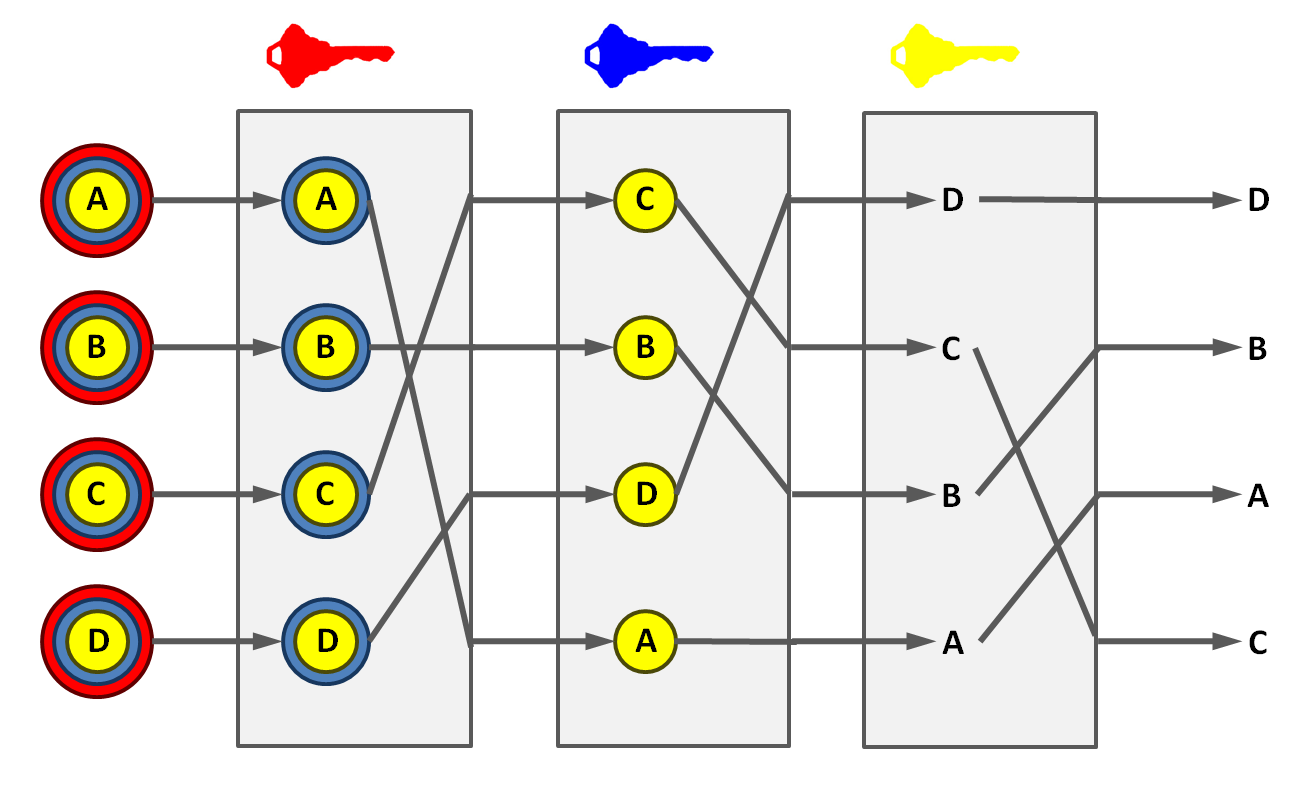
\includegraphics[width=\linewidth]{mixnet} \caption{An
%example decryption mixnet between three parties. Each message is encrypted by a
%sequences of public keys. Each party in the mixnet removes one layer by
%decrypting using its own key then outputs messages in a random order.}
%\label{fig:mixnet} \end{marginfigure}

\begin{marginfigure} 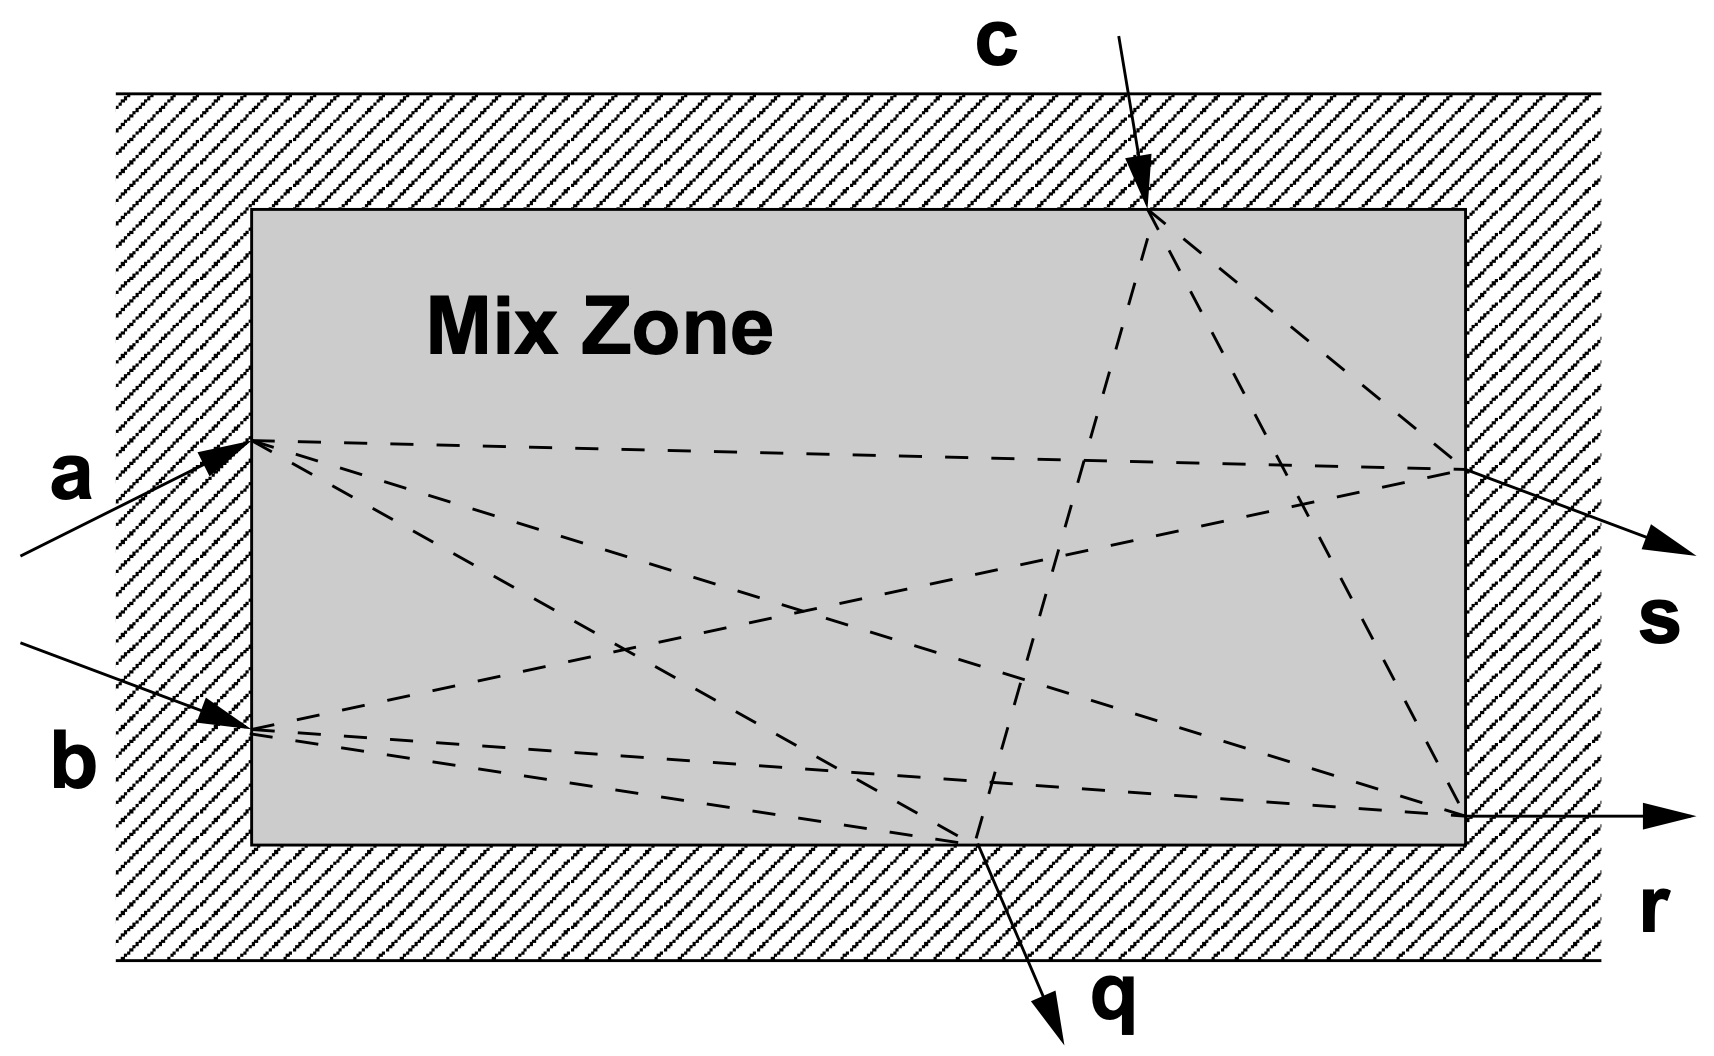
\includegraphics[width=\linewidth]{mixzone} \caption{
An illustration of a mix zone. Three trajectories, \textbf{a}, \textbf{b}, and
\textbf{c}, enter the zone and three trajectories \textbf{q}, \textbf{r}, and
\textbf{s} exit it. The paths from ingress trajectories to egress
trajectories is hidden and in this example gives 3-anonymity.
Source: \cite{freudiger2007mix}}
\label{fig:mixzone} \end{marginfigure}

In the scope of data sharing, mix networks can be used as a tool to allow third
parties to unlink individual identities from data sets. For example, a
concept of a \textbf{mix zone} was proposed as a way of achieving $k$-anonymity of
transit trajectories \cite{freudiger2007mix}. A mix zone would be a geographic,
high-traffic area where vehicle trajectories would not be logged. Upon leaving
a mix zone, vehicles would be assigned new identities. If at least $k$ vehicles
are in the mix zone at all times, each vehicle crossing through would be
$k$-anonymous. An example mix zone is illustrated in Figure \ref{fig:mixzone}.

\section{Advanced Cryptography}

Cryptography offers multiple technologies for privately computing over data,
including \textbf{zero-knowledge proofs}, secure \textbf{multiparty
computation}, and \textbf{homomorphic encryption}. There is a large body of work
on all of these technologies going back to at least 1982 with Yao's notion of
Garbled Circuits \cite{DBLP:conf/focs/Yao82b}.

Zero-knowledge proofs have had the most recent adoption and development by
digital currencies and will be discussed in the following section.

Until recently, real world applications of multiparty computation (MPC) were
limited to niche use cases like beet auctions \cite{DBLP:conf/fc/BogetoftCDGJKNNNPST09}.
However, the combination of protocol performance improvements, instruction-level
cryptographic primitives, and wider use of machine learning have led to
more MPC proposals for privacy-preserving machine learning, e.g.
\cite{DBLP:conf/ccs/BonawitzIKMMPRS17}.

Homomorphic encryption comes in two flavors: partial and fully.
\textbf{Partially homomorphic encryption} has been supported for decades by many
cryptosystems including RSA, ElGamal, and, most commonly, Paillier's
\cite{DBLP:conf/eurocrypt/Paillier99}. Recently, Google applied partially
homomorphic encryption for \textbf{Private Set Intersection} (PSI)
\cite{google-psi}.

Google is likely using PSI to privately join advertising data with external data
from credit card companies \cite{google-mastercard}. The application is to
attribute which ad impressions ultimately result in purchases, without either
party sharing its respective ad impression data or purchase data. Private set
intersection has a narrow scope, but is useful for summing common values between
two parties’ data sets without revealing their respective private data.

\textbf{Fully homomorphic encryption} (FHE) is a more powerful construction with
the promise of being able to compute arbitrary circuits over encrypted data. It
wasn't until 2009 \cite{DBLP:conf/stoc/Gentry09} that the first FHE scheme was
implemented; albeit one trillion times slower than a native computation. After a
decade of development, FHE performance has improved by orders of magnitude, but
is still too slow for general use. FHE is not commonly used in practice, so
standards for tools or protocols haven't emerged yet. However, companies
are working on building libraries, for example Microsoft Research released a FHE
library called SEAL \cite{sealcrypto}.

\section{Verifiable Data \& Verifiable Computation}
\label{verifiable}

An underlying motivation for data sharing is that one party may not trust
another to honestly report aggregate data. For example, regulatory agencies
conducting oversight may not trust aggregate data from service providers.
\textbf{Verifiable data structures} allow parties to verify whether an element
is a member of a set and, in some cases, whether it is a non-member.

A Merkle Tree \cite{merkle1979} is a classic verifiable data structure based on
hash functions and the underlying data structure of most blockchains.

\begin{marginfigure} 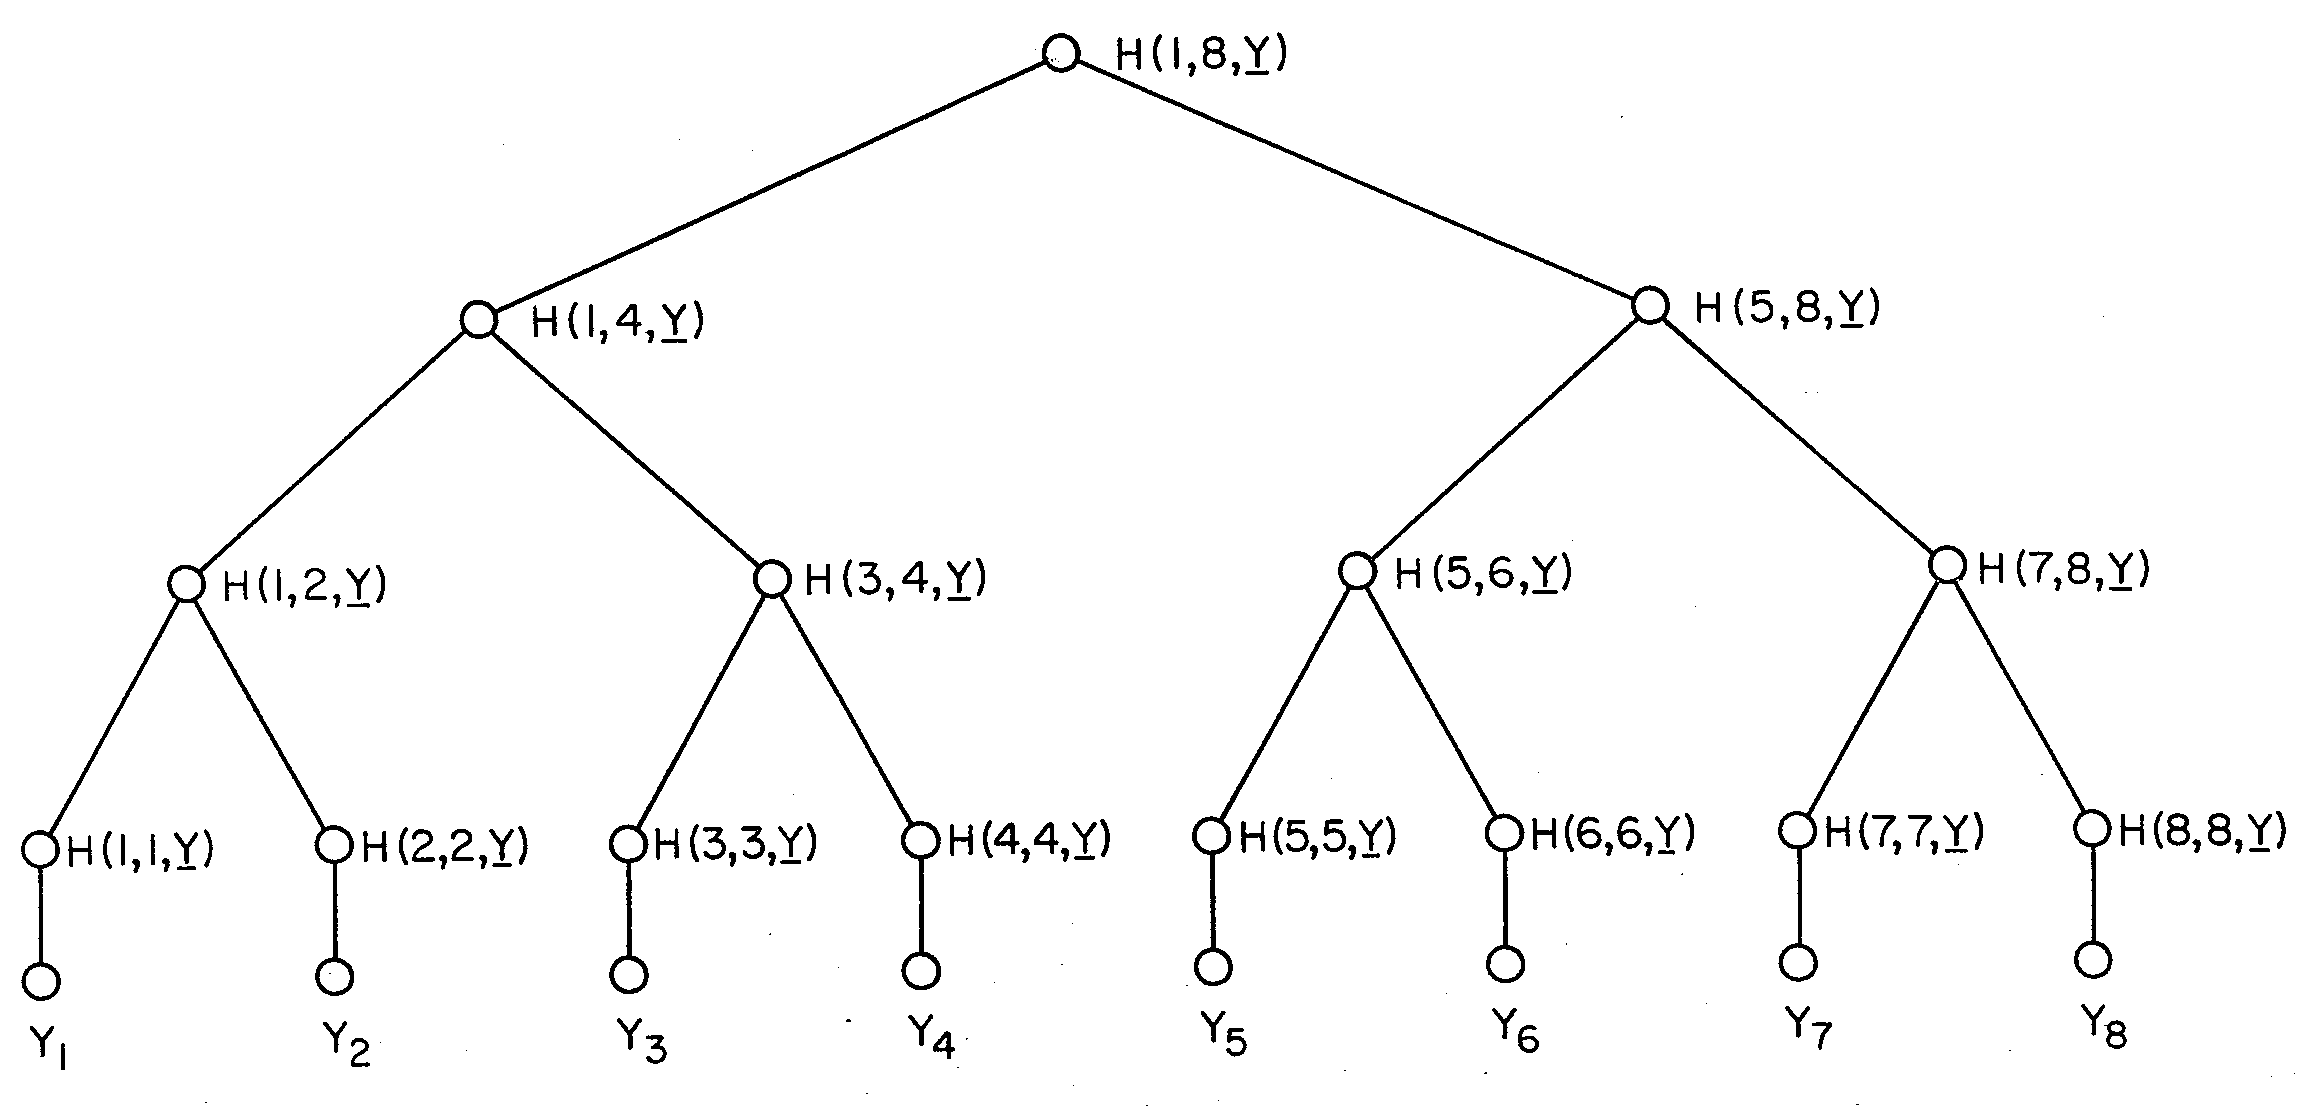
\includegraphics[width=\linewidth]{merkle} \caption{The
original Merkle tree from his 1979 patent application.} \label{fig:merkle}
\end{marginfigure}

Google’s Trillian \cite{google-trillian} verifiable data structures are used by
Google's Certificate Transparency (CT) project allow browsers to verify whether
a TLS certificate is a member of a known valid set. CT functions as a publicly
verifiable, immutable log similar to a blockchain, except for being
permissioned.

\textbf{Verifiable computation} coupled with a commitment log would allow a
private data owner to prove to another party that aggregate values were correctly
computed over private data. \textbf{Zero knowledge proofs} are a building block
to prove knowledge of some value without revealing what it is.

One zero knowledge technology with practical adoption are \text{zk-SNARK}s,
which stands for \textit{Zero Knowledge, Non-interactive Succinct ARguments of
Knowledge} \cite{DBLP:conf/sp/Ben-SassonCG0MTV14}. SNARKs are used by anonymous
digital currencies to prove that transactions reconcile without revealing the
participants or transaction amount. That is, SNARKs can prove a transaction
isn’t creating or destroying money without revealing who is getting paid.

The combination of a verifiable data structure and zero knowledge proof system
could make it unnecessary to share raw data in the first place. A publishing
party would commit to a log of ciphertexts or oblivious commitments before
sharing aggregated data. Then the publisher could prove that the inputs to the
data aggregation correspond to the committed values. An analog of this are
verifiable voting schemes where secret commitments to votes are published,
privately tallied, then available for audit to third parties.

\section{Summary Table}

This table summarizes the approaches discussed in this overview.
\textit{Lossy} means that shared data does not contain the entire original
data set or does not contain individual records. \textit{Complexity} is
generally how complex a technology is and \textit{maturity} is a general
sense of how much the approach has been adopted. \textbf{Bold} values are
desirable.

\begin{table}[ht]
  \centering
  \fontfamily{ppl}\selectfont
  \begin{tabular}{llll}
    \toprule
    Approach & Lossy? & Complexity & Maturity \\
    \midrule
    Minimization & N/A & \textbf{Low} & \textbf{High} \\
    Redaction & Yes & \textbf{Low} & \textbf{High} \\
    Aggregation & Yes & \textbf{Low} & \textbf{High}  \\
    Binning & Yes & \textbf{Low} & \textbf{High} \\
    $k$-anonymity & Yes & Medium & Medium  \\
    Tokenization & \textbf{No} & \textbf{Low} & High  \\
    Format-Preserving Encryption & \textbf{No} & Medium & Medium \\
    Differential Privacy & Yes & Medium & Medium \\
    Synthetic Data & Yes & Medium & \textbf{High} \\
    Secure Enclaves & \textbf{No} & High & Medium \\
    Mix Networks & \textbf{No} & High & Low \\
    Multiparty Computation & \textbf{No} & High & Low \\
    Partially Homomorphic Encryption & \textbf{No} & Medium & Medium \\
    Fully Homomorphic Encryption & \textbf{No} & High & Low \\
    Verifiable Computation & \textbf{No} & High & Low \\
    \bottomrule
  \end{tabular}
  \label{tab:normaltab}
\end{table}

\bibliography{priv-mech} \bibliographystyle{acm}

\end{document}
